
\chapter{ \uppercase {Residual Monte Carlo Treatment of the Time Variable}}
\label{sec:time}
Another extension and improvement for the HOLO method described in Sec.~\ref{} is the time discretization
of the transport equation.  We have
incorporated the time variable into the ECMC method to improve efficiency over IMC, while still preserving the
accuracy of MC integration.  The main area of interest is in producing more accurate
resolution of radiation wave-fronts in optically
thin regions, where particles transport a long distance over a time step. In such regions, the MC
integration of the time variable by IMC can produce greater accuracy than an implicit
Euler discretization, which can produce artificially fast propagation of radiation in
space.   A potential application where this accuracy is important is stellar atmosphere calculations.  It is
noted that no adaptive refinement in time is performed, so maintaining exponential convergence
may not be possible.  However, we still expect the residual MC formulation of the ECMC method
to show improvement in efficiency over standard MC.

In the remainder of this chapter, the inclusion of the time variable into the ECMC trial
space is detailed, along with modifications to particle tracking and the ECMC algorithm.
The process of sampling, tracking, and tallies particle histories in time
is detailed in literature\cite{wollaber_review,fnc,wollaber_thesis,cj_thesis}, but
sufficient details are provided in this chapter.  
Finally, a new temporal closure for the LO equations is given, and results are compared to IMC for accuracy and
efficiency.  

\section{Modifications to the HO equations}
\label{sec:time_ho}

Inclusion of the time variable $t$ in the trial space used by ECMC allows for no discretization of the
transport operator $\B L$.  The transport operator, applied to the continuous intensity
$I$, becomes
\begin{equation}
    \B LI(x,\mu,t) = \frac{1}{c}\pderiv{I}{t}  + \mu \pderiv{I}{x} + \sigma_t I
\end{equation}
The emission source is still treated with an implicit Euler discretization, which is
similar to the approximation made in IMC.  The ECMC algorithm specified in
Sec.~\ref{sec:???} does not need to be modified.  However, the residual
source and trial-space representation are modified to include $t$.   Each batch is still estimating the error in the
current projection estimate $\tilde I(x,\mu,t)$, but the time variable must be included in the inversion of the $\B L$
operator.  
\subsection{The Doubly-Discontinuous Trial Space in Time}

It is necessary to define a new trial space that includes the time variable so that we can explicitly evaluate the residual.
The time variable has a similar representation to the LDD trial space used for the
spatial variable
in Sec.~\ref{sec:lo_closure_LDDTRIAL???}, but the solution is a constant value over
the interior of the time step. This step, doubly-discontinuous (SDD) trial space is defined as
\begin{equation}\label{eq:time_space}
    \tilde I(x,\mu,t) = \left \{ \begin{array}{cl}
        \tilde I^{n}(x,\mu)  & \quad t = t^n \\ 
        \overline I(x,\mu)  & \quad t \in (t^{n},t^{n+1}) \\               
      \tilde I^{n+1}(x,\mu)   &  \quad        t = t^{n+1}
    \end{array}           \right.
\end{equation}
where we have used $\overline I$ to denote the time-averaged LDFE \emph{projection} in $x$
and $\mu$ of the intensity over the interior of the time step;  the beginning and end of
time step projections are denoted $\tilde I^{n}$ and $\tilde I^{n+1}$, respectively.   An
illustration of $t$ for the SDD trial space, over the $n$-th time step, 
is depicted in Fig.~\ref{fig:dd_time}.    There is a projection error in using the LDFE projection to represent the intensity between time steps.  However, with
sufficient noise reduction and mesh resolution, this should be an acceptable error
compared to the large statistical noise of standard MC.
\begin{figure}[H]
    \centering
    \begin{center}
%        \resizebox{0.4\textwidth}{!}{
        \begin{tikzpicture}[scale=0.882, every node/.style={transform shape}]
            \draw (1.0,4.0) node[fill,circle,inner sep=0pt,minimum
            size=4.2pt] {};
            \draw [->] (1.6,4.25) -- (2.4,4.25) node[anchor=west] {$t$};
            \draw (1.0,0.4) -- (1.0,0.6) node[below, pos=0.4] {$t^{n}$};
            \draw (5.90,0.4) -- (5.90,0.6) node[below, pos=0.4] {$t^{n+1}$};
            \node at (3.6,3.06) {$\overline{I}_{HO}(x,\mu)$};
            \draw [thick] (1.0,0.5) -- (5.9,0.5) node[anchor=north west] {};
            \filldraw[color=black, fill=white] (1,2.450) circle (2.1pt);
            \draw (1.0,2.45) -- (5.90,2.45);
            \filldraw[color=black, fill=white] (5.9,2.450) circle (2.1pt);
            \draw (5.9,1.6) node[black,fill,circle,inner sep=0pt,minimum size=4.2pt] {};
            \node[anchor=west] at (5.9,1.6) {${\tilde{I}_{HO}^{n+1}}$};
        \end{tikzpicture}
 %   }
    \end{center}
    \caption{Step doubly-discontinuous representation of $t$ for the HO solution.}
    \label{fig:dd_time}
\end{figure}

The SDD trial space provides a projection for all the desired unknowns to exactly produce the moment
equations, i.e., the time-averaged, end of time step, and previous time step intensities;
temporally, these are the only unknowns that appear in equations that have
been integrated over a time step to produce a balance statement.  Another benefit of this
trial space is it allows for infrastructure for computing the residual from the
time-discrete case to be used directly.  This trial space has one major drawback:
only particle histories that reach $t^{n+1}$ contribute to the estimation of $\tilde
\epsilon^{n+1}$, and thus $I^{n+1}$.  This is undesirable in optically thick problems.
%where not much correction to the time-variable is necessary and accuracy is limited by the 
%the BE discretization of the This is troubling, because in such problems you don't need much correction in
%the time variable.

REWRITE: Possibly move this to the future work section
Alternatively, an LDFE representation could be used in the time
variable. The linear representation would produce less noise because all particle tracks
contribute to the slope, rather than just those that reach the end of the time step,
although it would produce an approximate projection error for the end of time step
intensity that is not produced with a discontinuity at the end of the time step.  The
linear representation in time would also produce a more accurate reconstruction of the
scattering source in time.  However, a linear representation requires the sampling
algorithm to be significantly modified because the L$_1$ integral for computing the
residual magnitude is now significantly complicated by the tri-linear function.  A
possible way to sample this source is discussed in Appendix??? for completeness, but it has
not been rigorously investigated.

\subsection{Residual Source Definition and Sampling}

The residual is defined as $r = q - \B L \tilde I(x,\mu,t)$, where
\begin{equation}
    q=\left(\sigma_a a c (T_{LO}^{n+1})^4(x) + \sigma_s\overline\phi_{LO}\right)
\end{equation}
is a constant in time and provided by the LO solver. We have assumed a constant reconstruction for the scattering source
in time.
Evaluation of the residual with Eq.~\eqref{eq:time_space} for $I$ produces a uniform source in time, as well as a $\delta$-function source at the
beginning and end of the time step.  We write the residual source in terms of three components:
\begin{equation}
    r(x,\mu,t) = \overline r(x,\mu)  + r^{n}(x,\mu)\delta^+(t-t^{n}) +
    r^{n+1}(x,\mu)\delta^-(t - t^{n+1}),
    \quad t\in[t^{n},t^{n+1}]
\end{equation}

We will look at each component individually.  
The first residual term is a constant in time with representation
\begin{equation}
    \overline r(x,\mu) = q  - \mu \pderiv{\overline I(x,\mu)}{x} - \sigma_t \overline
    I(x,\mu)
\end{equation}
Evaluation of the above function produces both face and volumetric sources, similar to in
the discrete case.  To sample $x$ and $\mu$ from the face and volume distributions, the same rejection procedure
can be used as for Eq.~\eqref{eq:???} and detailed in~\cite{jake}.    The
time variable can then be sampled uniformly over the time step, i.e., $t=t^n + \eta \Delta
t$, where $\eta$ is a uniform random variable with support $(0,1)$.

The second source has definition
\begin{equation}
    r^{n}(x,\mu) = -\frac{1}{c}\pderiv{\overline{I}(x,\mu)}{t}\bigg|_{t=t^{n}}
    =-\frac{1}{c}\left(\overline I(x,\mu) - \tilde I^{n}(x,\mu)\right)
\end{equation}
This source is a LDFE space and angle volumetric source.
The rejection sampling procedure is used to sample $x$ and $\mu$.
All particles sampled from this source begin tracking with $t=t^{n}$.

The final source term is
\begin{equation}
    r^{n+1}(x,\mu) = -\frac{1}{c}\pderiv{\overline{I}(x,\mu)}{t}\bigg|_{t=t^{n+1}}
    =-\frac{1}{c}\left(\tilde I^{n+1}(x,\mu) - \overline I(x,\mu)\right).
\end{equation}
The source $r^{n+1}$ can be treated using the
same analytic treatment as the outflow face source in the LDD
trial space, detailed in Sec.~\ref{sec:???}; the source at the end of the time step is never sampled because its
contribution to $I^{n+1}$ can be analytically computed.  To treat the sources this way, the solution for $\tilde I^{n+1}(x,\mu)$ is
initialized to the value of $\overline I(x,\mu)$ before a batch of particles begins.
Then, error particles that reach the end of the time step, referred to as ``census''
particles, contribute a standard score to the projection $\tilde I^{n+1}(x,\mu)$.

With these definitions, it is thus only necessary to sample from two sources.  Using
composite-rejection sampling~\cite{shultis_mc}, a discrete probability distribution is
sampled to determine which source component to sample, followed by sampling of that
component.  The algorithm is
\begin{enumerate}
    \item Sample uniform random number $\eta$
    \item If $\eta < \|r^{n}\|_1/(\|r^{n}\|_1 + \|r^{n+1}\|_1)$:
    \begin{itemize}
        \item Sample from $r^{n}$ source using rejection sampling
        \item Sample $t$ uniformly over $(t^{n},t^{n+1})$.
    \end{itemize}
\item Else:
    \begin{itemize}
        \item Sample from $\overline r$ source
    \end{itemize}
\end{enumerate}
All L$_1$ integrals can be analytically integrated using the same numerics as in the
time-discrete case.  The systematic sampling algorithm, as described in
Sec.~\ref{sec:???}, can be applied similarly.  However, the choice of source is only make
locally over that space-angle element. In that case, the element is chosen systematically,
then the choice of $r^{n}$ or $\overline r$ is sampled.
REWRITE: Only discuss sampling of systematic case.

\subsection{Importance Sampling on Interior of Time Step}

As an attempt to reduce variance in the estimate of $\tilde \epsilon^{n+1}(x,\mu)$, we use
important sampling in the time variable.  Systematic sampling is still used for
determining the cell of interest, and sampling as described above is used to determine
which source is sampled, based on the appropriate probabilities described in the previous
section.  However, when the interior source $\overline r(x,\mu)$ is sampled, we use
importance sampling for the conditional sampling of the uniform time step.  The goal is to ensure that some
histories reach the end of the time step.  In order to do this, we sample from a modified
PDF such that a fraction $p_{end}$ of particles sampled from $\overline r(x,\mu)$ are born
with $t\in(t^{end},t^{n+1})$.  We define $t^{end}=t^{n+1}-M/(c\sigma_t)$, where $M$ is the desired
number of MFP of travel the particle will undergo from the end of
the time step (e.g., 2 or 3).  The weights of particles sampled from this
distribution must be modified to prevent source biasing.

The new PDF to be sampled from is
\begin{equation}
    f^*(t) = \left\{ \begin{array}{cl}
        \frac{\ds 1 - p_{end}}{\ds t^{end} - t^n} &\quad 0 < t < t^{end} \\ 
        \frac{\ds p_{end}}{\ds t^{n+1} - t^{end}} & \quad t^{end} \leq t < t^{n+1}  \\
        0 & \quad \text{elsewhere}\end{array}  \right.
\end{equation}
The original PDF is $f(t)= 1/\Delta t$, for $t\in(t^{n},t^{n+1})$.  Thus, using the
standard procedure for importance sampling\cite{shultis_mc}, the starting time $t_{\text{start}}$ is sampled from
$f^*(t)$, and then weights are multiplied by the factor
$f(t_{\text{start}})/f^*(t_{\text{start}})$.  This procedure is not perfect in that if a
particle is moving from an optically thin to an optically thick
region, it is not guaranteed to reach census. However, this case does not introduce bias.

\subsection{Tracking and Tallying in Time}

Because our LO equations will be integrated over the time step, we only need to
perform MC tracking for $t\in[t^{n},t^{n+1}]$.  
The initial time for the particle is
sampled as described in the previous section. In inverting the $\B L$ operator, particles
are tracked until they reach the end of the time step.  Path lengths are sampled or the
weight is exponentially attenuated as before (e.g., Sec.~\ref{sec:???}).  As a particle
travels from position $x_{o}$ to $x_{f}$, with direction $\mu$, the time is updated as 
\begin{equation}
    t^{f} = t^{0} + \frac{|x_{f} - x_{o}|}{c \mu}
\end{equation}
where $c$ is the speed of light. For analog path-length sampling, if $t^{f}>t^{n+1}$ then $t^{f}$ is adjusted to $t^{n+1}$
and the path length is adjusted accordingly.  For continuous weight deposition, particles
are only tracked until they reach $t^{n+1}$.  A proof that this process of tracking
particles is a MC solution to an integral equation that is exactly inverse to the $\B L$ operator is
detailed in~\cite{cj_thesis,shultis_paper_cj_cites???}.  

Tallies must be adjusted to account for the averaging over the time step, and to compute the
intensity at the end of time step.  To produced the time-averaged representation
$\overline I(x,\mu)$, requires estimators for the average, $x$, and $\mu$ moments of the
error, e.g.,
\begin{equation}
    \overline\epsilon_{x,ij} = \frac{1}{\Delta t} \frac{6}{h_j}
    \int\limits_{t^{n}}^{t^{n+1}} \!\!\dd t \!\!\!
    \int\limits_{\xl}^{\xr} \!\!\!\!\! \dd x
    \hspace{-0.081in}\int\limits_{\mu_{j-1/2}}^{\mu_{j+1/2}} \hspace{-0.107in} \dd \mu
    \;\left(\frac{x - x_j}{h_{i}}\right) \epsilon(x,\mu,t)
\end{equation}
with a similar definition for the average and $\mu$ moments.  The estimators are defined
as
\begin{equation}
    \hat{\overline \epsilon}_{x,ij} =\frac{1}{N_{hist}} \frac{6}{\Delta t h_i} \sum_{n=1}^{N_{hist}}
    \frac{s_n}{h_{i}h_{j}} w_j \left(x_c - x_i\right),
\end{equation}
where the magnitude of the weights produce the L$_1$ integral over all phase space, i.e.,
\begin{equation}
\sum\limits_{n=1}^{N} w_n = \| r(x,\mu,t) \|_1 \equiv 
    \int\limits_{t^{n}}^{t^{n+1}} \!\!\dd t \!\!\!
    \int\limits_{\xl}^{\xr} \!\!\!\!\! \dd x
    \hspace{-0.081in}\int\limits_{\mu_{j-1/2}}^{\mu_{j+1/2}} \!\!\!\!\dd \mu\;
    |r(x,\mu,t)|.
\end{equation}
Here, $x_c$ is the center of the $n$-th
path length, and $s_{n}$ is the path length for the $n$-th path length in the $x-\mu$ cell.

Moments of $I^{n+1}(x,\mu)$ must be estimated to represent the end of time step intensity.
For example, the $x$ moment for the $ij$-th cell of the error at the end of time step is
\begin{equation}
    \epsilon^{n+1}_{x,ij} = \frac{6}{h_i} \iint\limits_{\mathcal{D}_{ij}} \left(\frac{x
    - x_i}{h_i}\right) \epsilon(x,\mu,t^{n+1}) \dd x \dd \mu
\end{equation}
The estimators for these moments are a generalization of the census
tallies used in IMC~\cite{wollaber_review,wollaber_thesis}.  The tallies are based on the
definition of the intensity as $I(x,\mu,t) = c h \nu N(x,\mu,t)$ given in
Eq.~\eqref{???}, similar to collision estimators~\cite{shultis_mc,mcnp}.  The census estimator for the $x$ moment is
\begin{equation}
    \hat\epsilon^{n+1}_{x,ij} = \frac{1}{N_{hist}} \frac{6}{h_j h_i} \sum_{n=1}^{N_{hist}}
    c w_j  \left(x_{c} - x_{i}\right)
\end{equation}
Similar tallies are defined for the other space-angle moments. These tallies can be
exceptionally noisy because only particles that reach the end of the time step contribute.


\section{Closing the LO Equations in Time}

The LO equations must be closed in time consistently with the HO
equations.   Previous work has enforced
consistency in time by adding a local artificial source to the time-discretized LO
equations in each cell~\cite{holo_rh}.  This
source was approximated based on the difference between the exact HO integral of the time
derivative and the approximate representation in the LO equations. The advantage
of this form is that the LO solver exclusively deals in
time-averaged unknowns for the radiation terms in the equations.  However, if the problem
is strongly non-linear or the time-averaged and time-edge
values differ greatly, this may become unstable.

We will alternatively use a
parametric closure in the time variable, similar to the spatial closures discussed in the
Sec.~\ref{???}.  The time-integrated LO equations can be written exclusively in terms
of time-averaged unknowns.  This closure
produces LO equations that have the same numerical difficulty to solve as the BE,
fully-discrete LO equations, but
have the potential to preserve the accuracy of the MC integration in time, upon non-linear
convergence of the system.   A closure relation is used to eliminate
the end of time step moments present from the time derivative term.   We will investigate different parametric forms of the closure for robustness.   Once the time-averaged unknowns have been calculated,
the time closures can be used to convert the time-averaged unknowns to end-of-time-step
values.

REWRITE THIS SENTENCE
One potential benefit of the time closure parameters is that $\overline I^{HO}$ will be
most different from $I^{HO,n+1}$ in problems that are optically thin.  In such problems,
$\sigma_a$ is small, leading to an optically thin problem.  However, there may be
difficulties in the MPV problems where the problems are tightly coupled and nonlinear, but
can lead to a large change over a time step.

REWRITE: I think most of these paragraphs can be moved to intro

\subsection{Derivation of Time-Averaged Moment Equations}

The time-continuous radiation equations are integrated in space and angle the same as
before.  For example, the $L$ and $+$ moment equation is
\begin{multline}
    \frac{1}{c}   \pderiv{ }{t} \mom{\phi}^+_L - 2\left({\mu}_{i-1/2} I_{i-1/2}\right)^+ + \mom{\mu I}^+_{L,i} 
    + \mom{\mu I}^+_{R,i} +  \sigma_{t,i} h_i \mom{\phi}_{L,i}^{+} -  \frac{\sigma_{s,i} h_i}{2} \left( \mom{\phi}_{L,i}^{+} +
  \mom\phi_{L,i}^{-}\right) \\ = \frac{h_i}{2} \mom{\sigma_a a c T^4}_{L,i} 
\end{multline}
This equation is then integrated over the time step, and the emission source is assumed
implicit.  The same manipulations can be
performed on the streaming term to form angular consistency terms, but the weighting fluxes are now
time-averaged values.  Thus, the angular consistency terms are computed with $\overline I(x,\mu)$.  
The equations with time-averaged consistency terms are
\begin{multline}\label{eq:t_moml_ex}
    \frac{\mom{\phi}_{L,i}^{+,n+1} - \mom{\phi}_{L,i}^{+,n}}{c \Delta t}
    -2\overline {\mu}_{i-1/2}^{\,+} \overline \phi_{i-1/2}^{\,+} + \overline{\cur {\mu}}_{L,i}^{+}
  \mom{\phibar}_{L,i}^{+}
  +  \overline{\cur\mu}_{R,i}^{+}
  \mom{\phibar}_{R,i}^{+} +  \sigma_{t,i}^{n+1} h_i 
  \mom{\overline\phi}_{L,i}^{n+1,+} \\-  \frac{\sigma_{s,i} h_i}{2} \left( \mom{\phibar}_{L,i}^{+} +
  \mom{\phibar}_{L,i}^{-}\right) = \frac{h_i}{2} \mom{\sigma_a^{n+1} a c T^{n+1,4}}_{L,i},
\end{multline}
These equations are exact at this point.  The BE approximation is used for the temperature
terms in the material energy equations, but the radiation energy deposition is a
time-averaged valued.
REWRITE: Maybe add material energy equation

\subsection{Parametric Time Closure}
%\subsection{Alternative time discretization}
%\label{sec:time}
%
The closure relations in time are different than the closure relations for the spatial
variable because we do not have a slope in time.  The following closure is a modified diamond
relation:
\begin{equation}\label{eq:tc_diam}
    I^{n+1} = 2\gamma \overline{I} - I^{n}
\end{equation}
where $\gamma$ is the closure factor and $\overline{I}$ is the time-averaged
intensity.  A modified BE discretization can also be used:
\begin{equation}\label{eq:tc_avg}
    I^{n+1} = \gamma \overline{I}
\end{equation}

The chosen closure relation must be used to eliminate the unknowns at $t^{n+1}$ from each
of the LO moment equations, with the values from the previous time step taken as a known quantity.  Thus, it is necessary to have a closure relation for each moment and half
range, producing four closure parameters per spatial cell.  The closure relations for the
$L$ moment and the modified diamond relation are
\begin{equation}\label{eq:tc_diam_l}
    \mom{\phi}_{L,i}^{\pm,n+1} = 2 \gamma_{L,i}^{\pm}\mom{\overline\phi}_{L,i}^{\pm} -
    \mom{\phi}_{L,i}^{\pm,n}
\end{equation}
with equivalent definitions for the $R$ moment.  Substitution of the above equation into
Eq.~\eqref{eq:t_moml_ex}
\begin{multline}
    \frac{2}{c\Delta t}\left[ \gamma_{L,i}^{+} \mom{\phi}_L^{+,n+1} - \mom{\phi}_L^{+,n} \right]
    -2\overline {\mu}_{i-1/2}^{\,+} \overline \phi_{i-1/2}^{\,+} + \overline{\cur {\mu}}_{L,i}^{+}
  \mom{\phibar}_{L,i}^{+}
  +  \overline{\cur\mu}_{R,i}^{+}
  \mom{\phibar}_{R,i}^{+} +  \sigma_{t,i}^{n+1} h_i 
  \mom{\overline\phi}_{L,i}^{n+1,+} \\-  \frac{\sigma_{s,i} h_i}{2} \left( \mom{\phibar}_{L,i}^{+} +
  \mom{\phibar}_{L,i}^{-}\right) = \frac{h_i}{2} \mom{\sigma_a^{n+1} a c T^{n+1,4}}_{L,i},
\end{multline}
The other moment equations are analogously defined.  

The value of $\gamma_{L,i}^+$, $\gamma_{R,i}^+$, $\gamma_{L,i}^-$, and $\gamma_{R,i}^-$
can be computed by substituting the trial-space representation of $I^{HO}(x,\mu,t)$ into
Eq.~\eqref{eq:tc_diam_l} and its analogs.


\section{Computational Results}

We will test the time-closure in several characteristic cases.  The first case is a
near-void where the time-closure parameters will provide the most correction compared to a
Backward Euler discretization.  The second problem is the Marshak wave problem from
Sec.~\ref{sec:???}.  This problem is optically thick, so minimal time-correction is
needed, but there will likely be higher variance in the census tallies. We will compare to IMC
visually for accuracy to determine that we are converging towards the correct solution.
For the near void case the IMC solution is accurate because the material energy equation
is uncoupled.

\subsection{Near-Void Problem}

The problem specifics for this problem are a constant. We use the systematic sampling
algorithm and no biasing in time as the problem is optically thin. The material properties
are uniform throughout the 2.0 cm domain with $\rho c_v = 0.01374$ Jks cm$^{-3}$ keV$^{-1}$, $\sigma_a=10^{-6}$ cm$^{-1}$, and $\sigma_s=0$ \invcm.
The material and radiation are initially in equilibrium at a temperature of $0.01$ keV.  An isotropic incident intensity of 0.150 keV is applied
at $x=0$; the incident intensity on the right boundary is $0.01$ keV.  The simulation end
time is 0.003 sh.  
\begin{figure}[H]
  \centering
    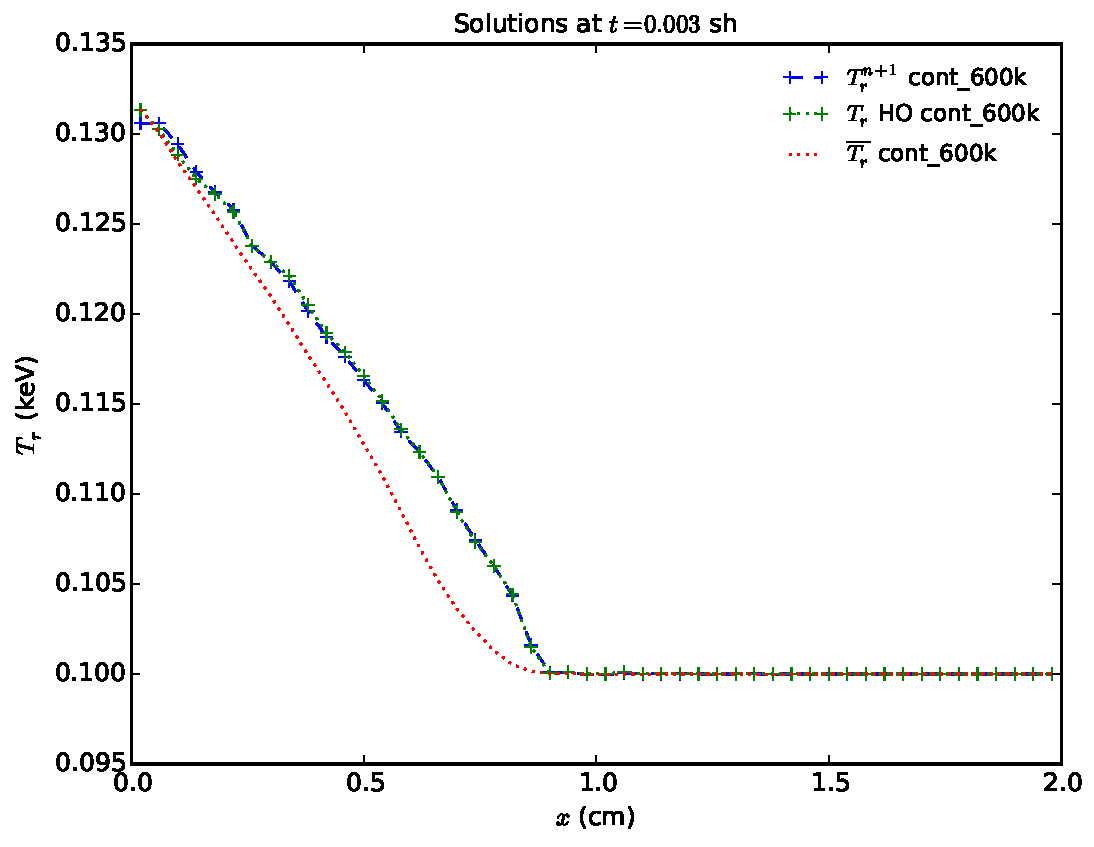
\includegraphics[width=0.65\textwidth]{void_imc_compare.pdf}
    \caption{\label{fig:void_imc_compare} Comparison of radiation energy densities of IMC
    and HOLO method for the HO time closure and a BE discretization.}
\end{figure}

A comparison of the cell-averaged radiation energy densities $E_r$ for IMC and the HOLO
method with the diamond-like HO time closure are depicted in Fig.~\ref{fig:void_compare},
both for the time-averaged solutions and end-of time step values in the final time step.
The end of time step values for the HOLO method with a BE discretization is also depicted.
For the HOLO results, three ECMC batches were performed with
a total of $3\times10^6$ histories per time step and the IMC results were generated with
$12\times10^6$ histories per time step.  The spatial mesh had 100 spatial cells and the
ECMC results used 20 $\mu$ cells.  

The MC treatment of the time
variable and the closure of the LO equations allow the results to correctly reconstrcutr
the wave-front of IMC.
time-continuous solutions are 

There is some visible mesh imprinting, in the form of
minor bumps, in the HOLO results
due to the projection of the solution between time steps. 

The census radiation temperatures are plotted in Fig.~\ref{fig:void_ecmc_temps} for two different
time step sizes.  By plotting
proportional to the fourth-root of the radiation energy density, there is more visible
noise.  This noise is small in comparison to the overall scale of the radiation energy
density, but it results from particles being born near the wave-front with a time sampled
near the beginning of the time step.  Negativities can occur out front of the wave.  In
the algorithm the average is set to the floor value and slopes to zero in such cells.  At
the smaller time steps, the noise is less visible because there is less inaccuracy in the
step approximation over the interior of the time step.  These inaccuracies should be
reduced by the linear time trial space. Causality is not strictly
preserved because you are sampling the error, so it is possible to have particles reach
the front of the wave front. This is not a bias, just insufficient sampling.

A comparsion for radiation temperatures with 1 and 3 batches is given in Fig.~\ref{blah}, which
reveals that there is substantial noise past the wave front for the 3 batches case.  This
noise is small relative to the scale of the solution in the wave-front, which is why it is not visible in the
mean intensity plots. This demonstrates one deficiency in this methdo that particles
sampled near the wave-front can potentially ahve a time near the beginning of the time
step and travel into the equilibrium region.  The solution is not biased however, if
sufficient samplign was performed there woudl be negative particles that canceled out this
error.  The residual MC case does not display this error as drastically because the guessed solution
takes on the form of the old solution, particles can not transport past what physics
allows, with the exception of some smearing due to the projection error incurred between
time steps.

We have computed FOM statistics using Eq.~\eqref{eq:fom} with 20 independent runs for each
configuration.  In general more particle histories are needed to produce an accurate
result.
\begin{table}[H]
\centering
\caption{\label{marshak_var} \textbf{Comparison of sample statistics for the Near-Void
    problem.   Simulation end time is $\mathbf{t=0.003}$ sh.}}
\vspace{-0.1in}
\begin{tabular}{|c|cc|cc|}\cline{2-5}
    \multicolumn{1}{c|}{}       & \multicolumn{2}{|c|}{\ss} &
    \multicolumn{2}{|c|}{\FOM} \\ \hline
hists./step   & IMC & HOLO-ECMC &  IMC & HOLO-ECMC   \\ \hline
   300,000
   1,000,000  & 3.40\%  & 0.28\% &  1    &  145      \\
  2,000,000    & 1.22\%  & 0.057\% & 0.93    &   422     \\ \hline
\end{tabular}
\end{table}


